Ce cycle désigne les principales étapes de développement du logiciel.
Le but de cette sécantation est de permettre la vérification du processus de développement.
Il comprend le plus souvent les étapes suivantes :
\begin{itemize}
        \item L'analyse des besoins et de la faisabilité du projet
        \item La conception
        \item Le codage
        \item Les tests
        \item La documentation
        \item La mise en production
        \item La maintenance
\end{itemize}
Le cycle de vie peut être modélisé de plusieurs manières (Figures \ref{fig:methv}  et \ref{fig:methv2}).
Nous utiliserons ici le modèle Agile puisqu'il implique le client, nous forçant à continuellement 
interagir avec lui. Il s'agit d'un modèle à la fois incrémental, itératif et adaptatif 
permettant un remaniement régulier du travail réalisé puisque le développement des tests et du logiciel 
sont effectués de manière synchrone.

    \begin{figure}[t]
        \centering
        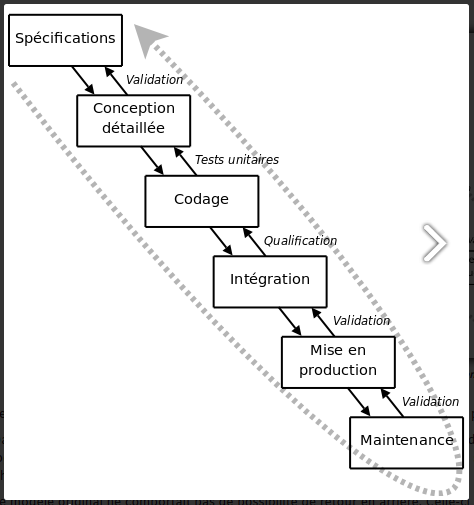
\includegraphics[scale=0.35]{images/Analyse_des_besoins/methcasc.png}
        \caption{Modèle du cycle de vie en cascade \cite{audibert2009uml}}
        \label{fig:methv}
    \end{figure}
    \begin{figure}[t]
        \centering
        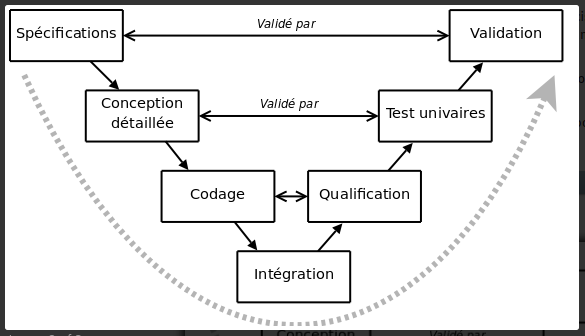
\includegraphics[scale=0.35]{images/Analyse_des_besoins/methv.png}
        \caption{Modèle du cycle de vie en V \cite{audibert2009uml}}
        \label{fig:methv2}
    \end{figure}